\section{Algoritmo 2: Dividir y Conquistar con OpenMP}
\label{sec:algo2_omp}

\subsection{Implementación y Selección de $n$}
Se implementó el algoritmo de dividir y conquistar en C++ utilizando paralelismo de tareas con \texttt{\#pragma omp task} sobre los cuatro cuadrantes independientes de la matriz resultado $C$. Dado que cada cuadrante $C_{ij}$ ocupa posiciones disjuntas de memoria, se evitan condiciones de carrera sin requerir sincronizaciones explícitas ni buffers temporales. 

Se seleccionó $n=256$ como tamaño de bloque de caso base. Esta elección se fundamenta en que un bloque de $256 \times 256$ doubles ocupa \SI{512}{\kibi\byte}, ajustándose a la capacidad de las memorias caché L2 privadas de ambos procesadores (\SI{1}{\mebi\byte}/core en PC1 y \SI{256}{\kibi\byte}/core en PC2) y generando 64 tareas a nivel de hoja, lo que permite un reparto equitativo entre $p \in \{1, 2, 4, 8\}$ hilos.

\begin{figure}[htbp]
    \centering
    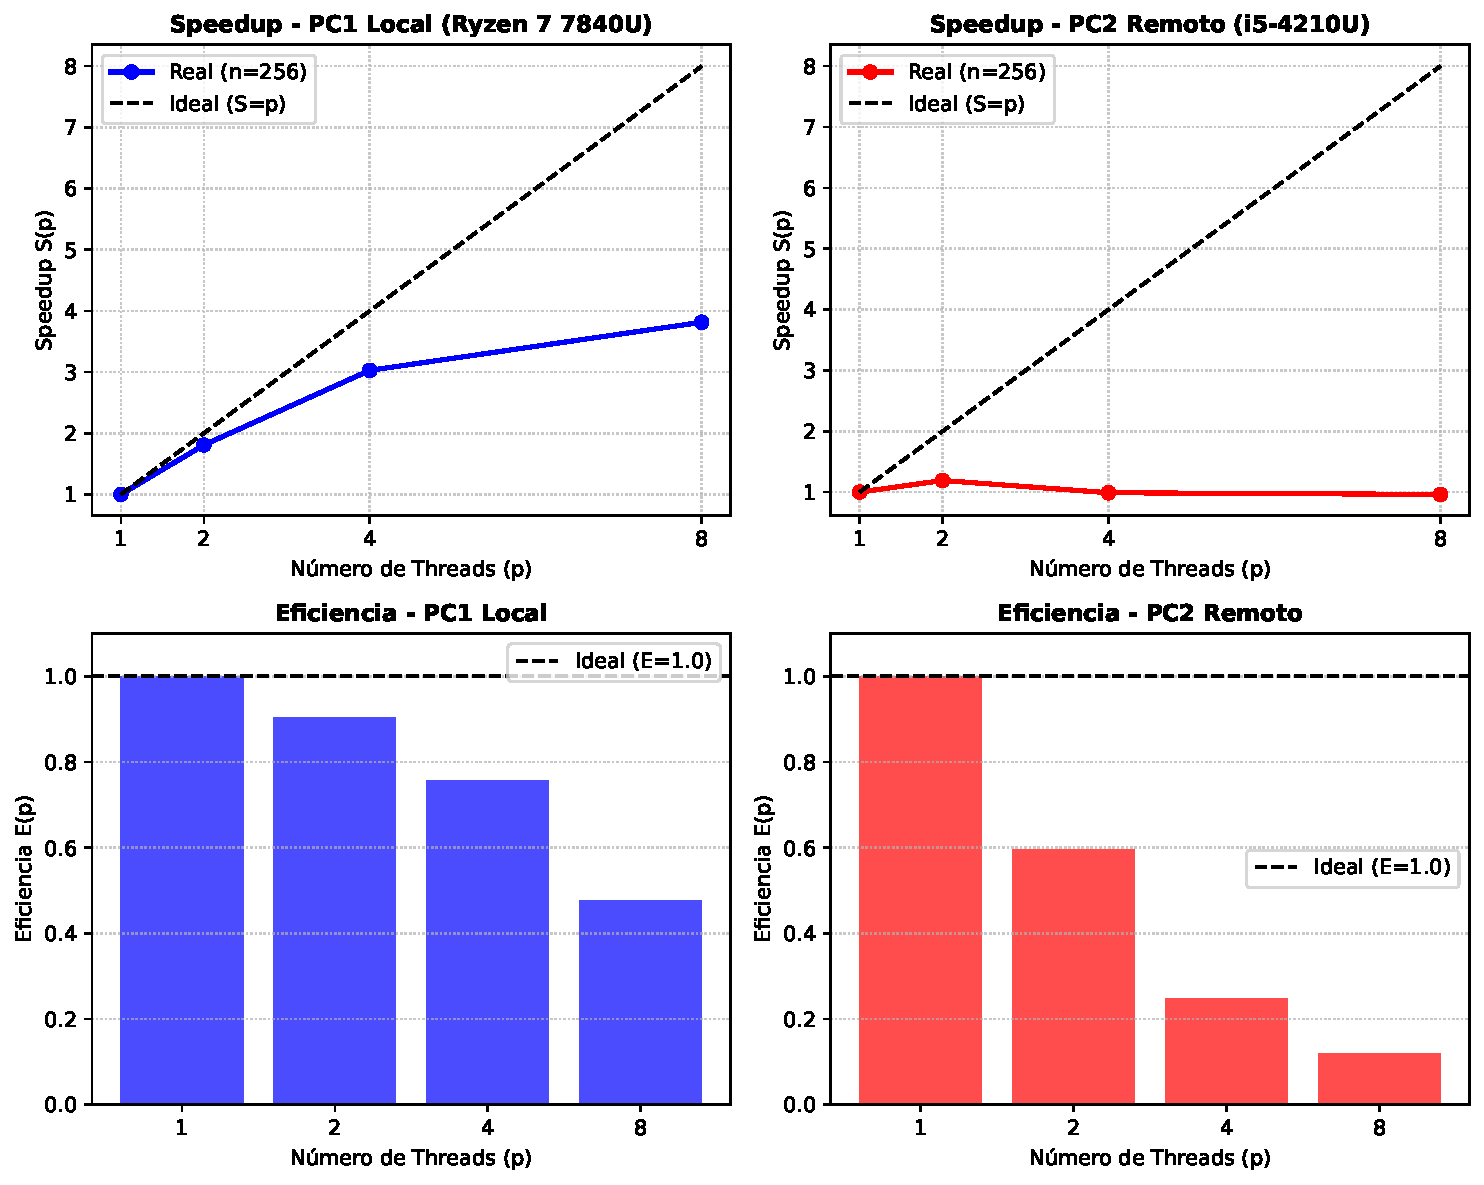
\includegraphics[width=\textwidth]{C/exp_c_plots.pdf}
    \caption{Resultados de Speedup y Eficiencia (Local vs. Remoto) para el Algoritmo 2 (Dividir y Conquistar, $n=256$).}
    \label{fig:exp_c_plots}
\end{figure}

\begin{table}[htbp]
\centering
\footnotesize
\setlength{\tabcolsep}{4pt}
\caption{Tiempos promedio (ms), Speedup $S(p)$ y Eficiencia $E(p)$ para el Algoritmo 2 ($N=2048, n=256$).}
\label{tab:resultados_c}
\begin{tabular}{r ccc ccc}
\toprule
& \multicolumn{3}{c}{\textbf{PC1 Local (AMD Ryzen 7 PRO 7840U)}} & \multicolumn{3}{c}{\textbf{PC2 Remoto (Intel Core i5-4210U)}} \\
\cmidrule(lr){2-4} \cmidrule(lr){5-7}
$p$ & Tiempo (ms) & Speedup $S(p)$ & Eficiencia $E(p)$ & Tiempo (ms) & Speedup $S(p)$ & Eficiencia $E(p)$ \\
\midrule
1 & 1195.60 & 1.0000 & 1.0000 & 4371.64 & 1.0000 & 1.0000 \\
2 & 661.41  & 1.8076 & 0.9038 & 3669.95 & 1.1912 & 0.5956 \\
4 & 394.84  & 3.0281 & 0.7570 & 4417.29 & 0.9897 & 0.2474 \\
8 & 313.49  & 3.8138 & 0.4767 & 4543.87 & 0.9621 & 0.1203 \\
\bottomrule
\end{tabular}
\end{table}

\subsection{Análisis}
En \textbf{PC1}, el algoritmo logra una eficiencia del \SI{90.4}{\percent} con $p=2$ y \SI{75.7}{\percent} con $p=4$, reduciendo el tiempo a \SI{313.49}{\milli\second} con $p=8$. En términos absolutos, el Algoritmo 2 es casi 4 veces más rápido que el Algoritmo 1 gracias a la explotación de la localidad espacial y temporal de la memoria caché. En \textbf{PC2}, el speedup alcanza su máximo en $p=2$ ($1.19\times$) y se degrada para $p \ge 4$ debido a la existencia de solo dos núcleos físicos reales y al estrangulamiento térmico (\emph{thermal throttling}) inducido por su bajo TDP (\SI{15}{\watt}).
